\chapter{绪论}

\section{课题背景及意义}
绿色能源已成为当今世界能源发展的主要趋势。未来人类可能会面对全球能源危机,发展绿色能源是能源发展惟一的出路。
各国政府纷纷制定了本国的绿色能源发展计划。在港口码头领域,绿色能源,清洁能源正发挥着越来越重要的作用。

船舶停靠码头时,装卸货物电气设备所需电力主要是从船舶电力系统来获取。船舶靠岸期间,用电是由船上的辅机组提供,
辅机发电会消耗化石燃料,主要是重油或者柴油。发电机组工作过程中,化石燃料的使用会排放诸如氮氧化合物,硫氧化合物,
和粉尘等一些污染物,会对港口空气质量造成一定的影响,同时发电机组会产生较大的噪声,影响港口附近人员的工作和
生活。

为了建立绿色港口,清洁港口,减少污染物的排放,船舶在停靠港口时,可以停止使用用柴油发电机组发电,
改用岸上电力系统提供所需电力。中国是世界上最大的航运国家,2020年,全球前20大集装箱港口中国仍占近半数,前10
大集装箱港口中有7个来自中国,中国港口货物吞吐量连年增长。根据国际海事组织(IMO)研究数据表明,2020年,全球
航运业需要4亿吨燃料,排放14亿吨$CO_{2}$,约占全球$CO_{2}$总排放量的$6\%$。保守的估计,我国每年靠港船舶
消耗的燃料油约为$70$万吨,船舶辅机发电的碳排量占港口总碳排量的40\%\~{}70\%\cite{SP1}。

岸电在美国西海岸已是强制性要求,在我国和一些亚洲国家尚在发展之中。我国交通部颁布的《船舶与港口污染防治专项行动实施方案》
(2015-2020年)对促进岸电发展发挥了巨大作用,截至2020年我国$90\%$的公务船舶、港作船舶靠泊时使用了岸电,
$50\%$的客滚、集装箱和邮轮专业化码头具有向船舶提供岸电的能力。港口应用岸电后,船舶靠港时污染物的排放
明显减少,港口环境得到了改善。应用船岸连接技术,对于港口地区的环境保护有重大的意义,
如果船舶岸电技术得到大力发展,所有靠港船舶都由岸电提供电力,那么既可以降低$30\%$的燃油成本\cite{SP2}和节省部分的维护成本,
也能够帮助港口实现IMO减排目标,为国家绿色可持续发展助力。

国家十四五规划,对碳排放,空气污染物的排放量作出了约束性的规定,推广使用岸电技术是保护港口环境,减排防污的一
大重要举措,对建设生态文明友好型的港口具有重大意义。表\ref{tab:岸电替代效益}中数据为中国沿海港口使用可再生能
源替代辅机发电的污染物和碳排放量对比,船舶靠港使用岸电后,微尘等颗粒物的排放减少了78\%,空气污染物$SO_{x}$、
$NO_{x}$的每\si{KW.h}排放量分别减少了74\%和80.1\%。结果表明,船舶靠港使用岸电的做法在节能和温室气体排放方面帮助
不大,但可以有效减少空气污染物的排放,在港口环境保护中的作用明显。

\begin{table}[!htp]
	\centering
	\caption[中国岸电替代辅机发电的减排表现]{中国岸电替代辅机发电的减排表现\cite{SP3}}
	\label{tab:岸电替代效益}
	\resizebox{\textwidth}{!}{
	\begin{tabular}{c}
		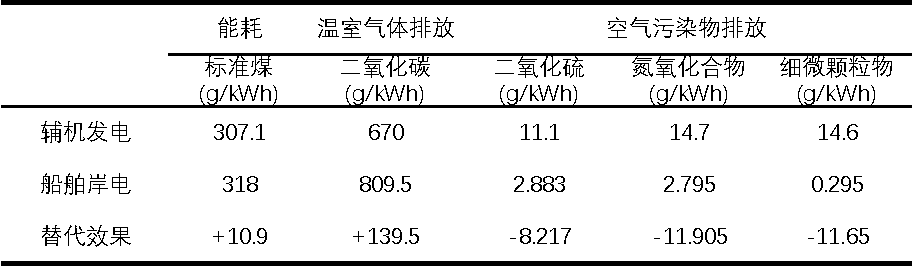
\includegraphics{chapter1/岸电替代效益.pdf} 
	\end{tabular}
	}
\end{table}

电气化,自动化,智能化是全球大趋势,工业过程、城市交通、供热和制冷在未来将由从$CO_{2}$零排放的绿色可再生能源获
得的电力来供电。到 2050年,全球发电容量预计将达到当前发电容量的两倍或三倍,岸电是我国在交通领域实现电气化的重要部分。

总之,船舶靠港停用辅机改用岸电是港口码头实现防污减排的首选方案,这在全球范围内取得了一定的共识。
其次,船舶辅机的发电效率并不是很高,改用岸电后,接入电网计价方便,具有良好的经济替代效益。
最后,发展岸电技术,提高港口自动化率,是中国制造的内在要求。未来,伴随着一带一路的发展,沿线国家的港口势必
会迎来更多的中国货船,推广中国岸电的技术,制定中国岸电技术标准显得十分必要。
中国在成为科技强国的路上,必须大力发展先进技术,在港口领域,我们要大力发展电气化,自动化和智能化的港口,
具体到电气化,则需要大力推广船舶岸电技术,推动船岸连接系统的发展与完善。


\section{船岸连接系统研究现状}
船岸连接技术解决的是港口污染和碳排放超标的问题,受这些问题的影响对该技术研究早在上世纪70年代就开始起步,
发展至今,该技术已经逐步发展完善与成熟,船岸连接系统的相关技术标准也正在趋于完善。
国内外都对船岸连接系统进行了研究与设计,由于国外起步较早,技术成熟且应用广泛,形成了一定的技术标准。
国内起步发展相对较晚,不过近年来随着绿色发展观念的深入人心,在国家的大力倡导下,中国岸电技术发展势头迅猛,
然而国内范围的船岸连接系统许多仍处在试验阶段,发展和推广应用的工作依然任重而道远\cite{SP4}。

\subsection{国外应用状况}
1989年瑞典哥德堡港率先应用船岸连接技术,由于当时的技术限制哥德堡港采用了低压(400V)岸电系统,
船岸连接技术的应用明显改善了港口环境状况。哥德堡港于2000年安装了ABB公司开发的一套高压岸电系统,这也使得哥德堡港成为了世界上
第一个应用高压岸电系统的港口。该系统的电压为6.6KV,容量为1250\si{KV.A},岸电的应用使得停泊船舶的污染物排放量减少了94\%-97\%
\cite{SP4},防治港口污染的作用显著。

2001年,美国朱诺港使用港口岸电向五艘改装的豪华游轮供电,标志着岸电技术在豪华游轮码头的首次应用。岸电系统的成功应用使其
在欧洲和美国引起了广泛的关注。2004年,美国洛杉矶港与中国集装箱船舶公司共同建造的7.5\si{MW}高压岸电系统建成投入使用\cite{SP5},
并计划于2014年在所有集装箱码头安装船舶岸电设施,这是岸电系统在集装箱码头的首次应用。

\begin{figure}[!htp]
	\centering
	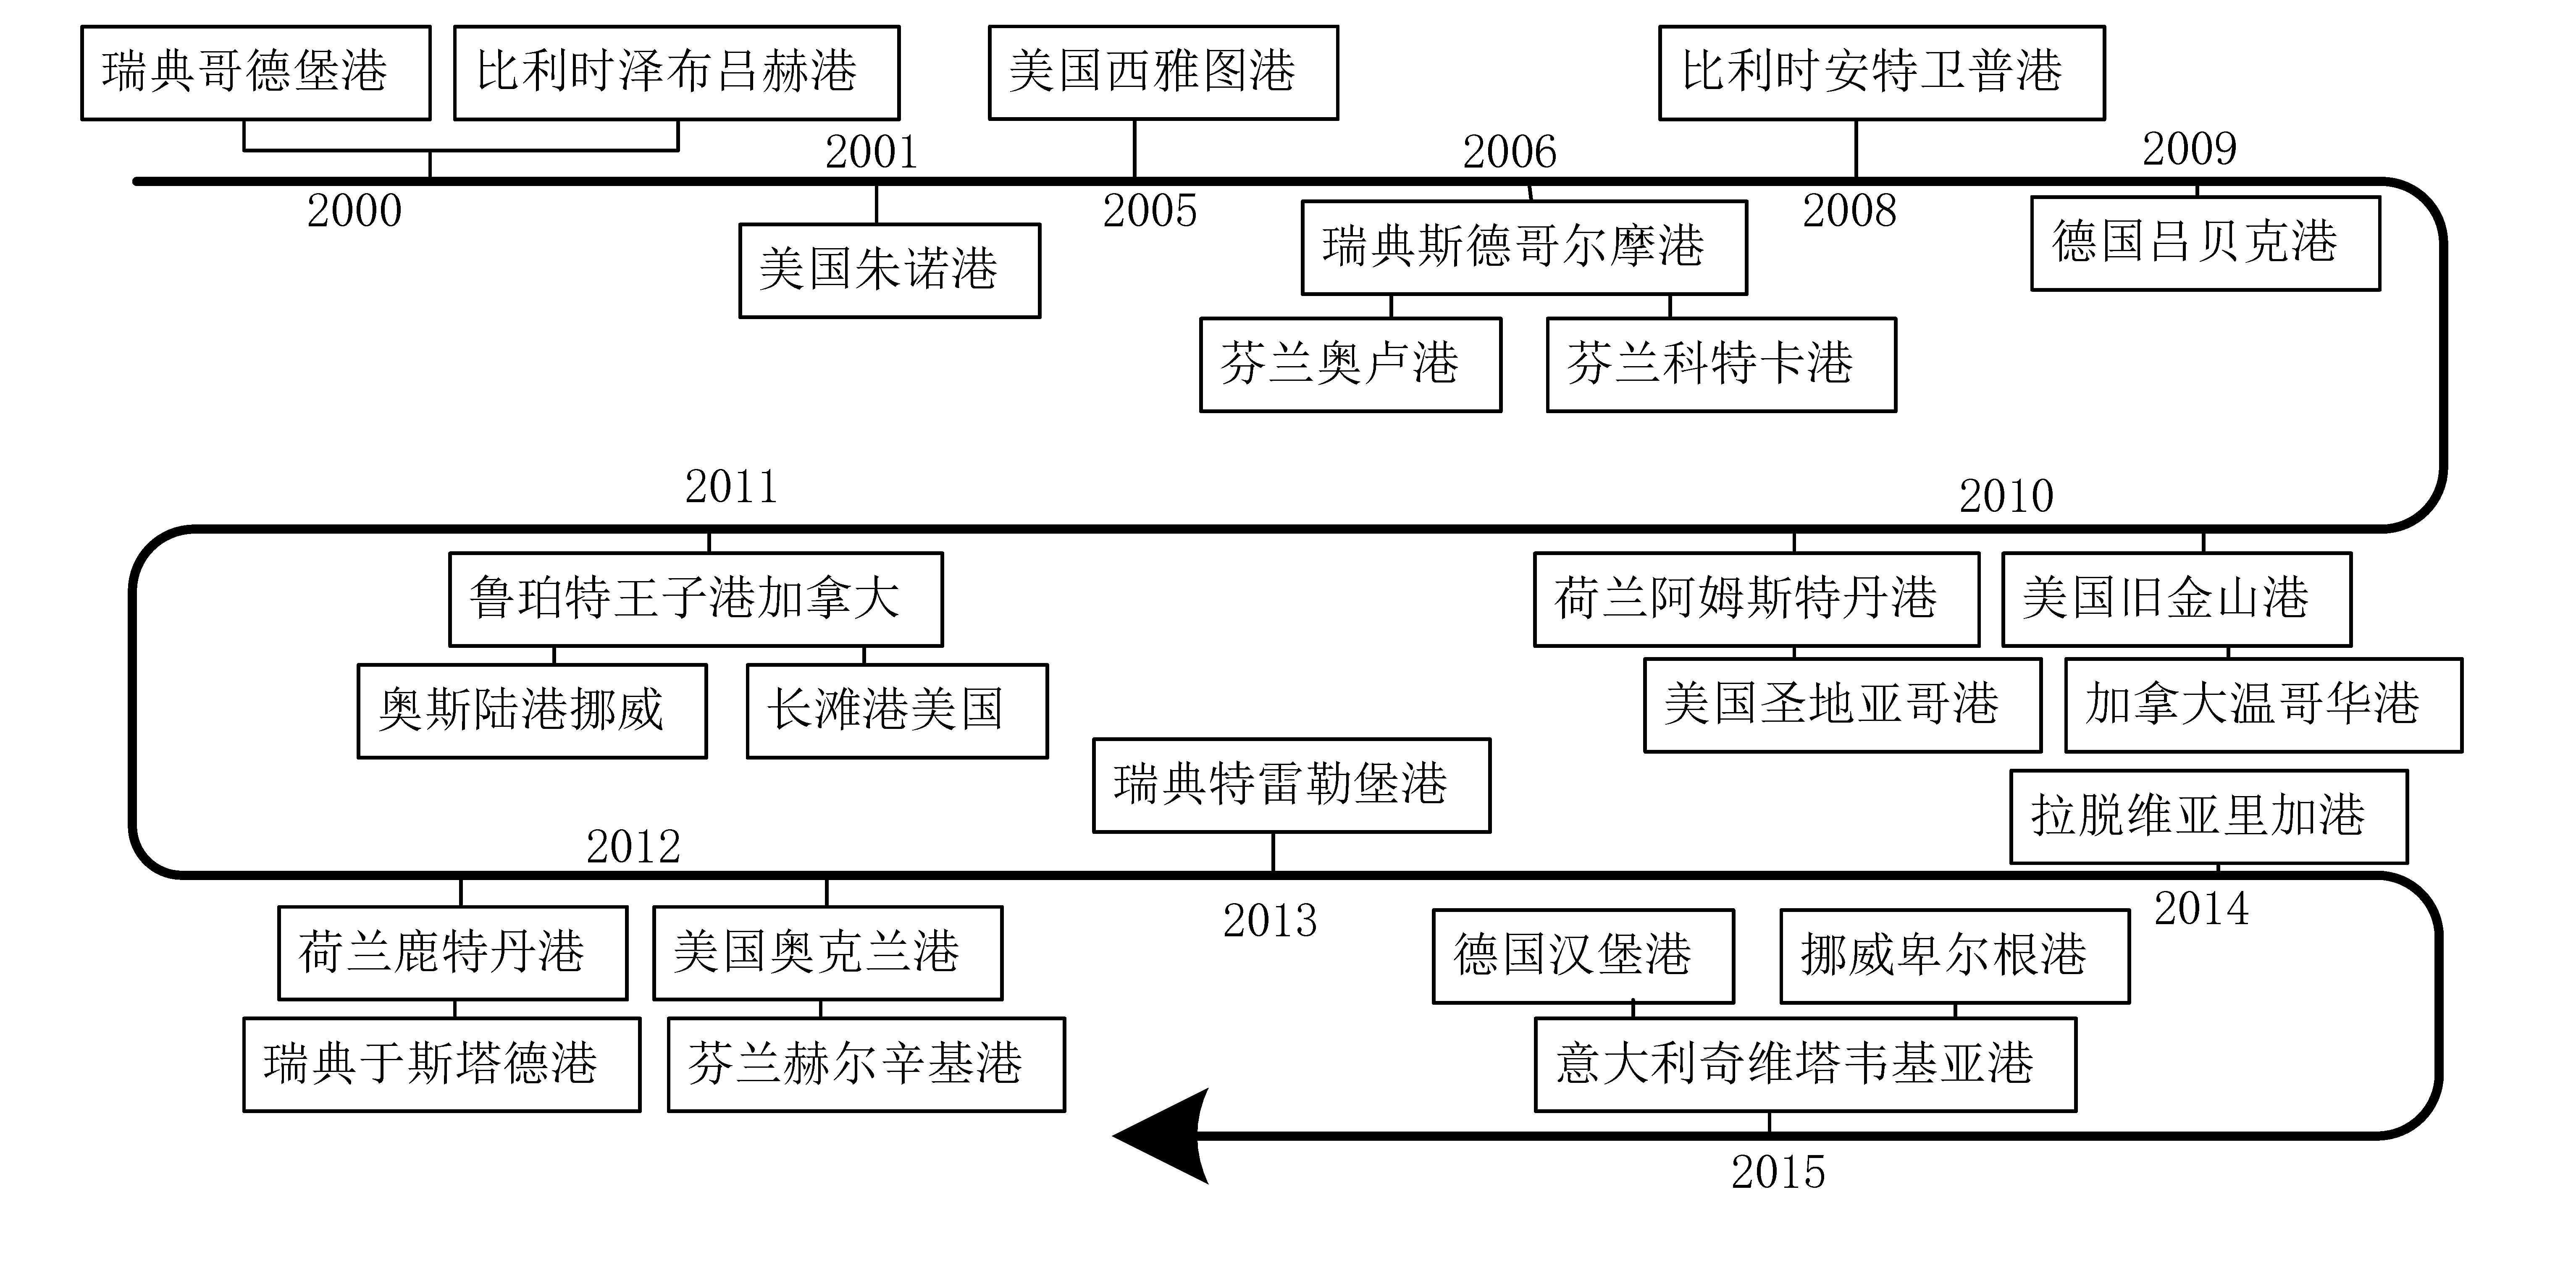
\includegraphics[width=\textwidth]{chapter1/国外应用岸电技术的主要港口.pdf}
	\caption{国外主要港口的岸电发展}
	\label{fig:国外主要港口的岸电发展}
\end{figure}

2009年,美国长滩港首次将岸电系统应用在石油码头,为大型油船提供港口岸电。2012年后,在纽约布鲁克林邮轮码头、安特卫普港集装箱码头、
吕贝克港等也安装了岸电系统。此外,国外诸如东京港、奥克兰港、纽约港、旧金山港等主要港口也正在计划或建设岸电基础设施\cite{SP6}。

图\ref{fig:国外主要港口的岸电发展},表示了国外主要港口的岸电发展和建设情况。总之,发达国家主要港口的岸电系统建设和应用已经比较普
遍,而且像ABB、西门子和凯福特一些西方发达国家的大公司拥有岸电系统总体建设的能力,他们拥有较大的技术领先优势,产品成熟而且
掌握大量岸电系统核心技术与专利,如凯福特的电源管理系统和快速连接头,ABB公司的静止频率变换器(PCS6000)\cite{SP5}。

\subsection{国内应用状况}

如图\ref{fig:国内主要港口的岸电发展}所示,我们可以看到近年来国内主要港口的岸电的建设情况。
我国最早对船舶岸电技术进行研究始于2005年,上海港开始对船舶岸电系统进行立项研究。2009年,我国第一个岸电系统
在青岛港建设完成,并在青岛港招商局集装箱码头为停靠船舶提供岸电,项目采用的是380V/50Hz的低压方案,容量仅为131.6\si{KV.A}。
2010年,上海外高桥码头10KV/50Hz岸电系统建设完成,拥有了对集装箱船供应岸电的能力。同年,连云港港建成了高压/低压岸电系统,
是国内首例实现了高压上船的项目,并成功将其应用在“中韩之星”客货两用船上\cite{SP4}。
此套岸电系统具有使用方便、整体轻巧,连接时间较短、实用性强等特点,获得了节能减排岸电专项奖和绿色港口技术认定\cite{SP8}。
后于2011年9月,连云港港为“富强中国”号开发了另一套船舶岸电系统,仍采取高压上船方案。

\begin{figure}[!htp]
	\centering
	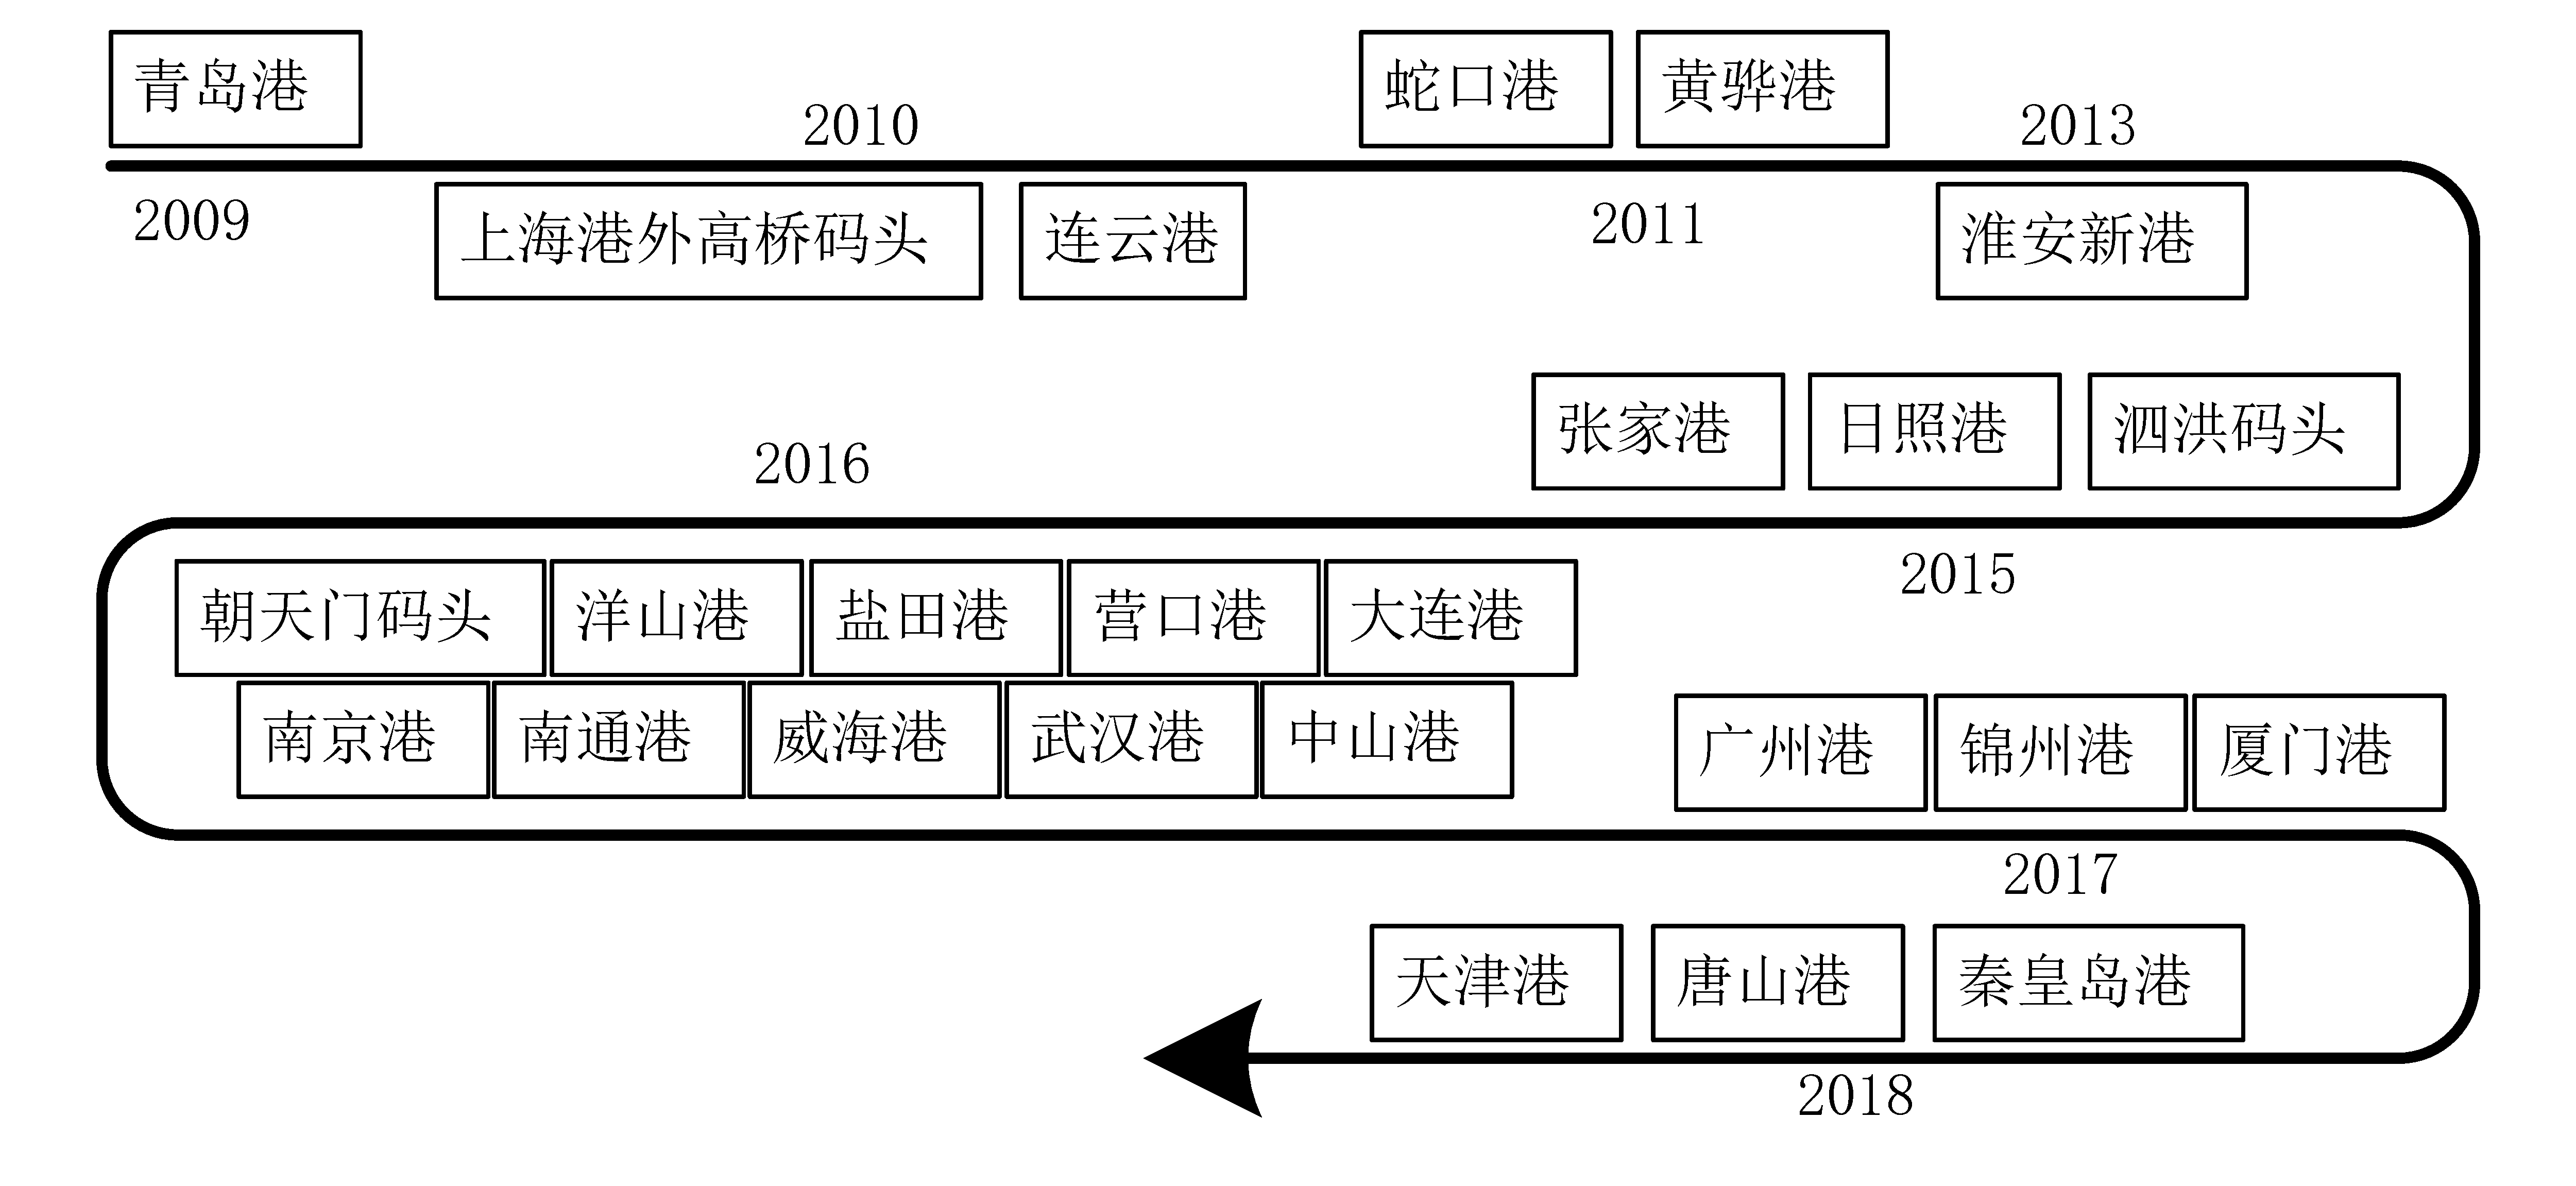
\includegraphics[width=0.9\textwidth]{chapter1/国内应用岸电技术的主要港口.pdf}
	\caption{国内主要港口的岸电发展}
	\label{fig:国内主要港口的岸电发展}
\end{figure}

2012年,深圳蛇口集装箱码头完成了对低压和高压岸电系统的建设工作;
2013年,国内首次实现带电并网的岸电系统——神华集团高压上船岸电项目,完成调试\cite{SP8};
2014年,天津港太平洋码的“太平洋东二、东四泊位岸基船舶供电项目”建设完成,输入10KV/50Hz经变换后输出6.6KV/60HZ的交流电;
2015年,日照港建成了第一套民用高压岸电系统\cite{SP9},同年泰州靖江新华港岸电系统开始为散货船供电;
2016年,盐田港由德国西门子研发的高压岸电项目建成,项目设计容量3000KW,预计能够实现年电能替代量
150万\si{KW.h},减排约1000吨。同年5月,舟山港与国网公司合作的舟山港项目正式投运,采用高压上船方案,设计容量为
2和3\si{MV.A},可为船舶提供6.6KV/60Hz与6KV/50Hz的交流电\cite{SP10}。

2017年,交通运输部水运局发布的《港口岸电布局方案》计划要于2020年实现泊位100\%的岸电覆盖率,对促进我国岸电系统的应用发挥了重要作用。
2018年,日照港对2个泊位进行的岸电改造项目建成,到2018年底国内已建成约3700个岸电设施,覆盖约5200个供电泊位。
2019年,大铲湾码头实现了100\%的泊位岸电覆盖率,是我国华南地区首个实现岸电100\%覆盖率的集装箱码头\cite{SP11}。
截至2019年底,全国已建成港口岸电设施5400多套,覆盖泊位7000多个(含水上服务区),总体完成率达81\%\cite{SP12}。

\begin{figure}[!htp]
	\centering
	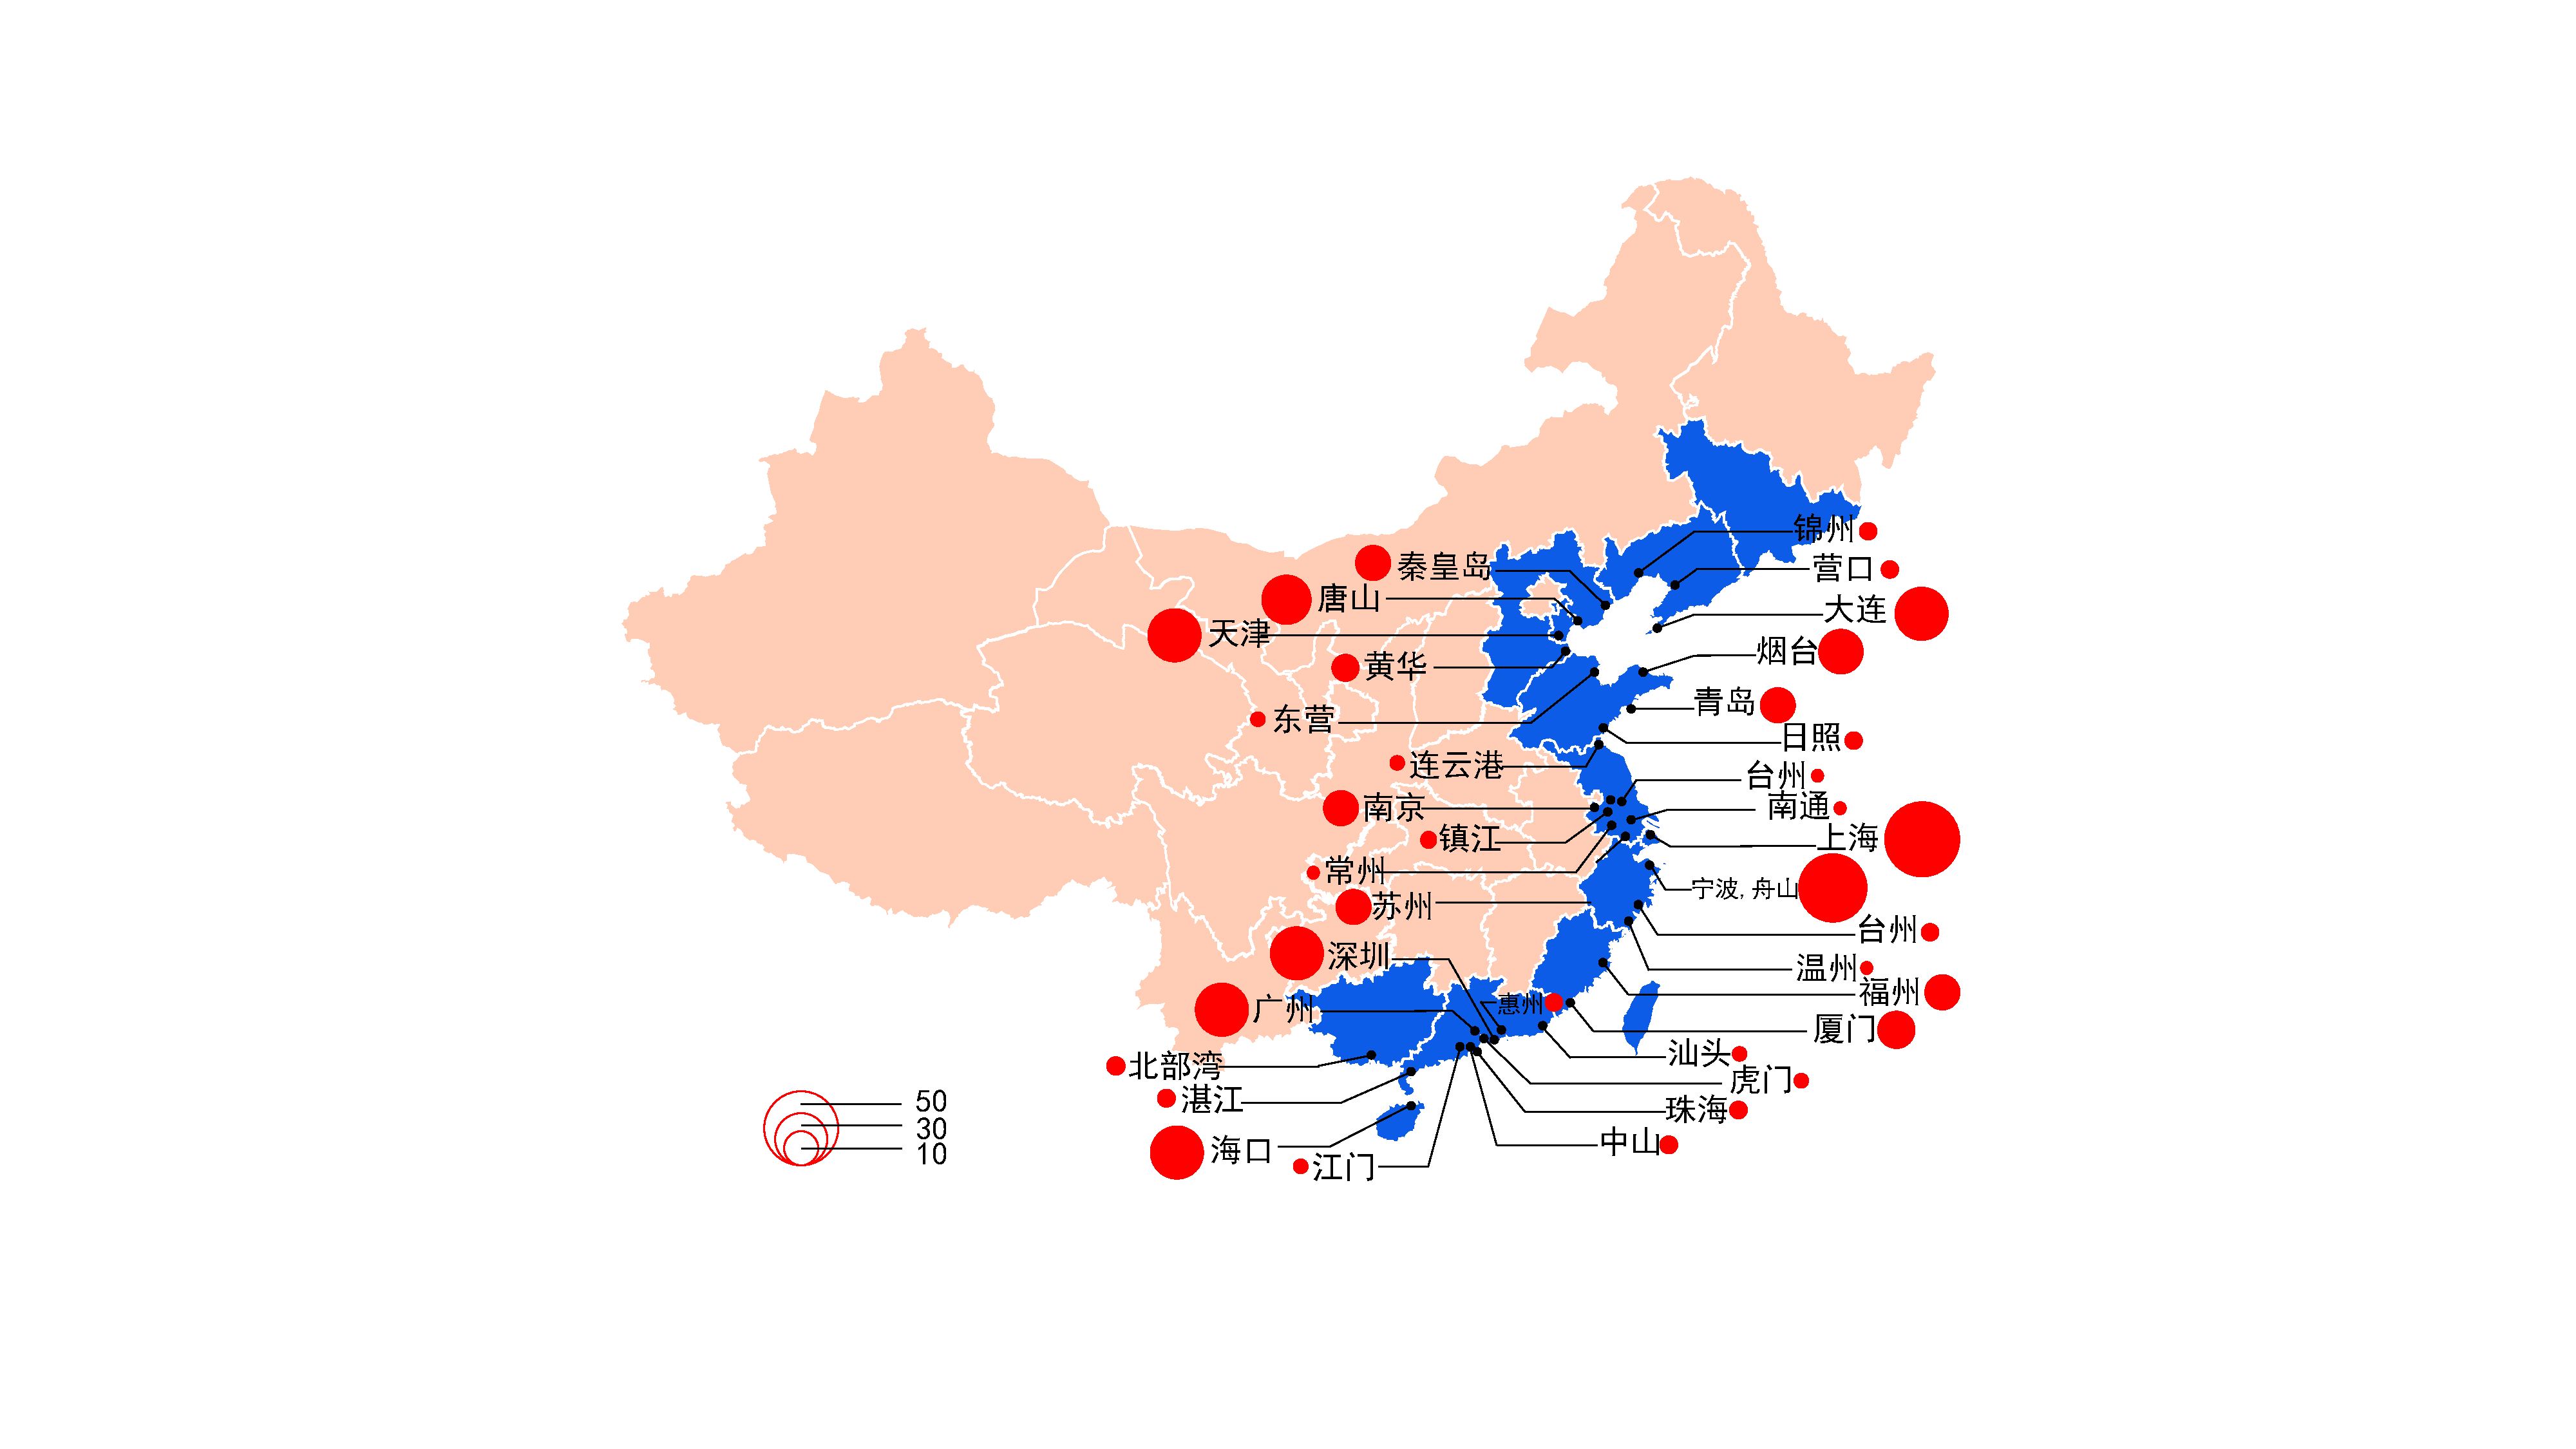
\includegraphics[width=0.9\textwidth]{chapter1/中国岸电分布图.pdf}
	\caption{ 2020年中国岸电分布图}
	\label{fig:中国岸电分布图}
\end{figure}

2020年中国的岸电建设取得了阶段性的成果,由于西方国家的工业进程总体领先我国,其对船岸连接技术的早研发早应用使得其目前仍
处于行业领先地位。我国船岸连接技术应用起步晚,岸电普及率相对较低,近年来在交通运输部等政府部门与国网公司等企业的大力倡导
和积极推动下,国内一些港口已经具备了提供岸电能力。

据公开数据统计,截至2020年底集装箱船、滚装客船、邮轮、客船(3000吨以上载重)和干舱(50000吨以上载重)泊位
的岸电系统分布情况如图\ref{fig:中国岸电分布图}所示。近年来我国岸电系统的发展迅速,国家重视程度高,可以说我国的岸电系统发展和应用正在如火如荼的进行着,当然
也存在着一些发展的问题如,泊位不足,标准制定等问题,但是中国拥有较大的市场容量,发展前景广阔。

\subsection{国内外岸电标准}

1983年,国际标准化组织(ISO)了ISO6812:1983 Preview Roll on/Roll off ship-to-shore connection,规定了滚装船的岸电设计标准。
这是第一个岸电系统领域的标准,也一直被沿用至今,后于2008年,ISO对该标准进行了重新审订\cite{SP4}。
表\ref{tab:国外相关标准的制定情况}中给出了国外岸电相关标准的制定情况与部分内容。
\begin{table}[!htp]
	\centering
	\caption[国外相关标准的制定情况]{国外相关标准的制定情况}
	\label{tab:国外相关标准的制定情况}
	\resizebox{0.95\textwidth}{!}{
	\begin{tabular}{c}
		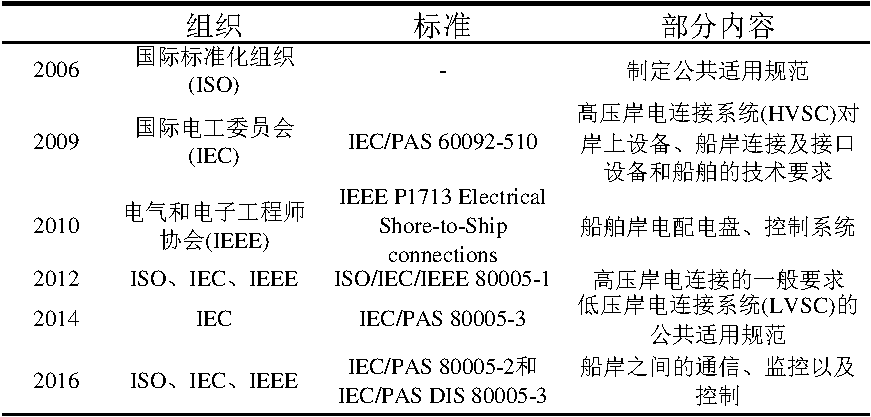
\includegraphics{chapter1/国外相关标准的制定情况.pdf} 
	\end{tabular}
	}
\end{table}

相比之下国内的岸电系统标准制定工作起步较晚,我国国内岸电系统领域相关标准的制定一定程度地依赖于国际标准\cite{SP4},
2005年,中国曾经派出代表参加了IEC 60092-510岸电标准的制定。近年来,我国交通部和国网公司大力倡导建设港口岸电系统,
国网公司下属许多单位从事着岸电系统和设备研发与生产,民营企业也逐渐加入到岸电系统的设计与研发的工作。同时,岸电标准
的制定也在逐步完善之中。交通部水运科学研究院等单位制定了《码头船舶岸电设施工程技术规范》,以及国网电力科学院等单
位制定了岸电系统、用电计量等一些列相关的企业标准\cite{SP14}。表\ref{tab:国内相关标准的制定情况}为岸电系统中
国标准的制定情况。

\begin{table}[!htp]
	\centering
	\caption[国内相关标准的制定情况]{国内相关标准的制定情况}
	\label{tab:国内相关标准的制定情况}
	\resizebox{0.95\textwidth}{!}{
	\begin{tabular}{c}
		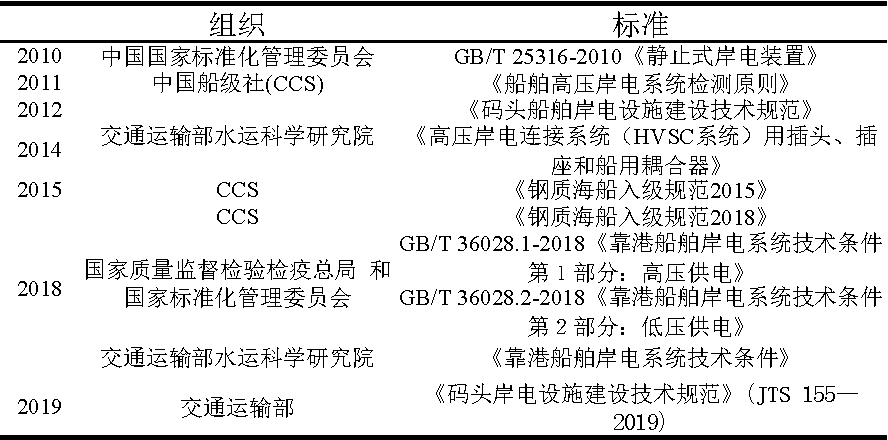
\includegraphics{chapter1/国内相关标准的制定情况.pdf} 
	\end{tabular}
	}
\end{table}

\section{论文研究内容及工作}
本文的研究目标旨在深入研究船舶岸电系统,并在此基础上设计船舶岸电并网控制的算法,以满足并网需求,做好保护功能
系统。使岸电系统可以实现港口岸电与船舶电网的无缝切换、负载的快速平稳转移以及相应的保护功能。本文的主要工作内容如下:

第一章,

第二章,

第三章,

第四章,

第五章,

第六章,


